
\section{Error Reporting}
\label{inference:errors}
In a constraint based inference algorithm, the natural way to include error reporting is to add justifications to each of the constraints extracted from the source program. These justifications can be maintained as the graph is reduced, and if we encounter an error we can use the justification to determine why the conflicting constraints were added to the graph. This approach is outlined by Wand \cite{wand:finding-type-errors}, and elaborated by Duggan \cite{duggan:explaining-type-inference}, Stuckey \cite{stuckey:improving-type-error-diagnosis} and Heeren \cite{heeren:top-quality-error-messages}. We will give an overview of the general ideas, and focus on how we manage the constraints that are specific to Disciple.

Consider the $\isuccDelay$ program from \S\ref{System:Effects:purification}

\code{
	\mc{2}{$\isuccDelay \ ()$} \\
 	$ \ = \ \kdo$	& $x = 5$ \\
               		& $y = \isucc \ @ \ x$ \\
			& $\dots$ \\ 
			& $x := 23$ \\
			& $\dots$
}

This program has a purity conflict. The binding for $y$ creates a suspension that will read the value of $x$, but later in the program this value is updated. This implies that the value of $y$ will depend on when it is forced, which is a program behaviour we take as being invalid. Here are the syntax trees for the three statements in the do-block, after desugaring:

\begin{center}
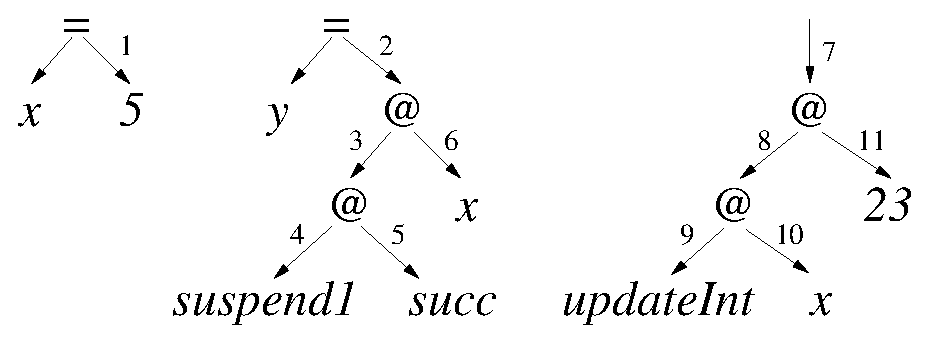
\includegraphics[scale=0.5]{3-Inference/fig/errors/suspend-succ.eps}
\end{center}

After extracting type constraints and solving them, we are left with a type graph containing the following equivalence classes:

\vspace{-1ex}
\begin{tabbing}
MMMMM	\= MM 	\= MM 		\= MMMMMMMMMM 		\= MM \kill
	\> *1	\> $\sim$	\> $s_x, \ a, \ s_1 \ s_6, \ s_{10}$		
				\> $= \ \iInt \ r_1$ 
	\\
	\> *2	\> $\sim$	\> $s_y, \ b, \ s_2$	
				\> $= \ \iInt  \ r_6$ 
	\\
	\> *3	\> $\sim$	\> $s_3$		
				\> $= \ s_x \lfuna{e_2 \ c_2} \ s_y$ 
	\\
	\> *4	\> $\sim$	\> $s_4$
				\> $= \ s_5 \lfuna{e_3 \ c_3} s_3$ 
	\\
	\> *5	\> $\sim$	\> $s_5$
				\> $= \ s_x \lfuna{e_5 \ c_5} s_y$\\
	\> \qq \dots \\
	\> \ !1	\> $\sim$	\> $e_5, \ e_6$
				\> $\tme \ \iRead \ r_1$ 
	\\
	\> \ !2 \> $\sim$	\> $e_7, \ e_9$
				\> $\tme \ \iRead \ r_{10} \lor \iRead \ r_1$
	\\
	\> \qq \dots \\
	\> \ $\Diamond$1 \> $\sim$ \> $\iPure \ e_5$ \\
	\> \ $\Diamond$2 \> $\sim$ \> $\iConst \ r_1$ \\
	\> \ $\Diamond$3 \> $\sim$ \> $\iMutable \ r_1$
\end{tabbing}

This graph contains an obvious type error. $\Diamond$2 contains a constraint that requires $r_1$ to be constant, while $\Diamond$3 contains a constraint that requires it to be mutable. As discussed in \S\ref{Core:Witnesses}, we cannot convert this example to a valid core program because there is no way to construct witnesses for both of these constraints at once. Unfortunately, the \emph{reason} for this error is not so obvious. It would be unhelpful for a compiler to simply report that it ``cannot create core witnesses'', or that ``$\iConst \ r_1$ conflicts with $\iMutable \ r_1$''. Neither of these messages help us determine what part of the program caused the error, or suggest how we might resolve it.

\subsection{Constraint justifications}

As mentioned previously, we track the source of type errors by attaching justifications to each of the constraints from the program. For example:

\begin{tabbing}
MMMMM	\= MMMM 		\= MMMMMMMMMMM 		\= MMMMMMMMM		\= MM \kill
	\> $s_{4u}$	\> $= s_5 \lfuna{e_3 \ c_3} s_3$		\> $| \ i_1$ 
	\\[0.5ex]
	\> $s_{4d}$ 	\> $= \rINST \ s_{\isuspend}$ 			\> $| \ i_2$
	\\[0.5ex]
	\> $s_{4u}$	\> $= s_{4d}$					\> $| \ i_3$
	\\[0.5ex]
	\> $s_5$	\> $= \rINST \ s_{\isucc}$			\> $| \ i_4$
	\\[0.5ex]
	\> $s_9$	\> $= \rINST \ s_{\iupdateInt}$			\> $| \ i_5$
	\\[0.5ex]
	\> $i_1$	\> $= \iIApp \ 3 \ \isuspend \ \isucc$ 
	\\
	\> $i_2$	\> $= \iIVar \ 3 \ \isuspend$
	\\
	\> $i_3$	\> $= \iIUseDef 3 \ \emptyset$
	\\
	\> $i_4$	\> $= \iIVar \ 3 \ \isucc$
	\\
	\> $i_5$	\> $= \iIVar \ 5 \ \iupdateInt$
	\\
	\> \dots
\end{tabbing}

We now write value type constraints as $s = \tau \ | \ i$, where $s$ is a type variable, $\tau$ is a type, and $i$ is a \emph{source information variable}. In this presentation we will refer to source information as just ``information''. We extend region, effect, closure and type class constraints in a similar way. Information variables are bound to information expressions in separate constraints. Information expressions are built with \emph{information constructors} such as $\iIApp$ and $\iIVar$. 

We give information constructors informal, descriptive kinds:

\code{
	$\iIApp$ 	&	$:: \trm{num} \to \trm{exp} \to \trm{exp} \to \trm{info}$ \\
	$\iIVar$ 	&	$:: \trm{num} \to \trm{var} \to \trm{info}$ \\
	$\iIUseDef$ 	&	$:: \trm{num} \to \trm{Set info} \to \trm{info}$
}

$\iIApp$ takes a line number and two expressions. It produces information that says a particular constraint is due to the application of these two expressions, on that line of the source program. $\iIVar$ produces information that says a constraint is due to the use of a particular variable. $\iIUseDef$ produces information that says a constraint is due to the fact that the definition of a variable must match its use. The first argument of $\iIUseDef$ is a line number as before, but the second argument is a set of other information expressions. We will see how this works in a moment. 

We now discuss how to record source information in the type graph representation. For constraints involving a constructor, we can take the information variable from the constraint, and use it to annotate the constructor as it is placed into an equivalence class. When performing an instantiation due to an $\rINST$ constraint, the information variable on the $\rINST$ constructor is propagated to all the new constructors created during the instantiation. For example, after adding the above constraints to the type graph and performing the instantiations we get:

\begin{tabbing}
MMMMM	\= MM 	\= MM 		\= MMMMMMMMMM 		\= MM \kill
	\> *1	\> $\sim$	\> $s_{4u}$		
				\> $= \ (s_5 \lfuna{e_3 \ c_3} s_3)^{i_1}$
	\\
	\> *2	\> $\sim$	\> $s_{4d}$
				\> $= \ (s_{41} \lfuna{e_{4d} \ c_{4d}} s_{42})^{i_2}$ 
	\\
	\> *3	\> $\sim$	\> $s_{41}$		
				\> $= \ (a \lfuna{e_{41} \ c_{41}} \ b)^{i_2}$ 
	\\
	\> *4	\> $\sim$	\> $s_{42}$
				\> $= \ (a \lfuna{e_{42} \ c_{42}} \ b)^{i_2}$ 
	\\
	\> \ !1	\> $\sim$	\> $e_5$
				\> $\tme \ (\iRead \ r_1)^{i_2}$ 
	\\
	\> \ $\Diamond$1 \> $\sim$ 	\> $(\iPure \ e_{41})^{i_2}$ \\
	\> \ $\Diamond$3 \> $\sim$ 	\> $(\iMutable \ r_2)^{i_4}$ 
	\\
	\> \ $\circ$1 \> $\sim$	\> $i_1$ 	
				\> $= \ \iIApp \ 3 \ \isuspend \ \isucc$ \\
	\> \qq \dots 
\end{tabbing}

Note that we have used $\circ$ to identify the equivalence classes that hold source information expressions. For a constraint of the form $s_{4u} = s_{4d} \ | \ i_3$, assuming that $s_{4u}$ and $s_{4d}$ are not already in the same class, adding this constraint to the graph may result in types being unified. As we wish to track the reason for this unification, we modify the reduction rule for unification so that it combines the information about the types being unified:

\clearpage{}
\begin{tabbing}
M \= MMMMMMMM \= M \= MMMMMMMMMM \= MMMMMMMMMM \= MMMM \kill
	\> (unify fun info)	
		\> $\{$ \> $s_1 = s_2 \ | \ i_1,$  \\
	\>	\> 	\> $s_1 = a_1 \lfuna{e_1 \ c_1} b_1 \ | \ i_2$,
			\> $s_2 = a_2 \lfuna{e_2 \ c_2} b_2 \ | \ i_3$ \\
	\>	\>	\> $i_1 = \iIUseDef n \ \emptyset$ \\
	\>	\> $\}$ 
	\\[1em]
	\> \qq $\vvdash$ 
		\> $\{$	\> $s_1 = s_2 \ | \ i_1,$ \\
	\>	\>	\> $s_1 = a_1 \lfuna{e_1 \ c_1} b_1 \ | \ i_4$ \\
	\> 	\>	\> $a_1 = a_2 \ | \ i_4,$ \> $b_1 = b_2 \ | \ i_4$ \\
	\> 	\>	\> $e_1 = e_2 \ | \ i_4,$ \> $c_1 = c_2 \ | \ i_4$ \\
	\>	\>	\> $i_1 = \iIUseDef n \ \emptyset$ \\
	\>	\>	\> $i_4 = \iIUseDef n \ \{ i_2, \ i_3 \}$ \\
	\>	\> $\}$	 
\end{tabbing}

The rule for unification of data types is similar. The new information constraint $i_4 = \iIUseDef n \ \{ i_2, \ i_3 \}$ records why the value, effect and closure constraints in the conclusion of the rule were added to the graph. It also contains the information variables from both types that were unified. Returning to our example, we use this new unification rule to add the constraint $s_{4u} = s_{4d} \ | \ i_3$ to the type graph:
\begin{tabbing}
MMMMM	\= MM 	\= MM 		\= MMMMMMMMMM 		\= MM \kill
	\> *1	\> $\sim$	\> $s_{4d}, \ s_{4u}$
				\> $= \ (s_5 \lfuna{e_3 \ c_3} s_3)^{i_6}$
	\\
	\> *3	\> $\sim$	\> $s_{41}, \ s_{5}$		
				\> $= \ (a \lfuna{e_{41} \ c_{41}} \ b)^{i_2}$ 
	\\
	\> *4	\> $\sim$	\> $s_{42}$
				\> $= \ (a \lfuna{e_{42} \ c_{42}} \ b)^{i_2}$ 
	\\
	\> \ $\circ$1 \> $\sim$	\> $i_1$ 	
				\> $= \ \iIApp \ 3 \ \isuspend \ \isucc$ \\
	\> \ $\circ$2 \> $\sim$ \> $i_2$	
				\> $= \ \iIVar \ 3 \ \isuspend$ \\
	\> \ $\circ$6 \> $\sim$	\> $i_6$ 	
				\> $= \ \iIUseDef \ 3 \ \{ i_1, \ i_2 \} $ \\

	\> \qq \dots 
\end{tabbing}
Unfortunately, although the \emph{set} representation contains full information about why a particular constraint is present, in our type graph representation some of this information is lost. Since we attach source information to constructors only, we have no way of adding a constraint like $s_1 = s_2 \ | \ i_1$ to an empty graph without losing the information variable $i_1$. For example, doing so yields:
\begin{tabbing}
MMMMM	\= MM	\= MM		\= MMMMMMMMMMM 		\= MM \kill
	\> *1	\> $\sim$	\> $s_1, \ s_2$ 	\> $= \bot$  
\end{tabbing}
On the left of the $=$ we have the list of variables in this equivalence class, with the canconical name $s_1$ appearing first. This list represents a substitution, where all occurrences of $s_2$ in the graph should be replaced by $s_1$. We have recorded this bare fact, but have lost the reason \emph{why} such a substitution should take place. For this reason we will stick with the constraint set representation for the rest of this section.

\clearpage{}
\subsection{Tracking purity errors}
Returning to the $\isuccDelay$ example from \S\ref{inference:errors}, we can track the source of the purity error by modifying the reduction rules for purity constraints:

\begin{tabbing}
	M \= MMMMMMMMM \= M \= MMMMMMMMMMMMMMM	\= MMMMMMMMM \= MMMMM \= MMMMMMM \kill
	\> (purify info)	
		\> $\{$ \> $e_1 \tme \iRead \ r_1 \ | \ i_1$, 
		\> $\iPure \ e_1 \ | \ i_2 \ \}$ 
	\\[1em]
	\> \qq $\vvdash$	
		\> $\{$	\> $e_1 \tme \iRead \ r_1 \ | \ i_1$, \> $\iPure \ e_1 \ | \ i_2$, \\
	\>	\>	\> $i_3 = \iIPurify \ r_1 \ i_1 \ i_2$, \> $\iConst \ r_1 \  | \ i_3$ $\}$

\end{tabbing}

\begin{tabbing}
	M \= MMMMMMMMM \= M \= MMMMMMMMMMMMMMM 	\= MMMMMMMMM \= MMMMM \= MMMMMMM\kill
	\> (purify trans info)	
		\> $\{$	\> $e_1 \tme e_2 \ | \ i_1$, 	
		\> $\iPure \ e_1 \ | \ i_2 \}$ 
	\\[1em]
	\> \qq $\vvdash$	
		\> $\{$	\> $e_1 \tme e_2 \ | \ i_1$, 
			\> $\iPure \ e_1 \ | \ i_2$, \\
	\>	\>	\> $i_3 = \iIPurifyTrans \ e_1 \ i_2$,
			\> $\iPure \ e_2 \ | \ i_3$ \ $\}$ 
\end{tabbing}

The (purify info) rule is an extension of (purify) from \S\ref{inference:type-classes}. The resulting $\iConst \ r_1$ constraint is now tagged with an information variable $i_3$. The constraint $i_3 = \iIPurify \ r_1 \ i_1 \ i_2$ says that $\iConst \ r_1$ arose from the purification of a read effect on region $r_1$. It also includes the information variables from the associated effect and purity constraints. We modify the (deep purify) rule in a similar manner.

The (purify trans info) rule extends (purify trans) from \S\ref{inference:type-classes}. The resulting $\iPure \ e_2$ constraint is tagged with a variable $i_3$, and the information constraint $i_3 = \iIPurifyTrans \ e_1 \ i_2$ records the variables in the premise of the rule. $\iIPurifyTrans$ constraints can be used by the compiler to find the original source of a purity constraint.  For example, consider the following set:
\begin{tabbing}
		MM \=	M 	\= MMMMMMMMMM \= MMMMMMMMMMMM \=  \kill
	\>	$\{$ 	\> $e_1 \tme e_2 \ | \ i_1,$ 		
	\\
	\>		\> $e_2 \tme e_3 \ | \ i_2,$ 	
	\\
	\>		\> $e_3 \tme \iRead \ r_1 \ | \ i_3,$ 
			\> $i_3 = \iIVar \ 3  \ \isucc,$ 
	\\
	\> 		\> $\iPure \ e_1 \ | \ i_4,$ 	
			\> $i_4 = \iIVar \ 3  \ \isuspend,$ 
	\\
	\>		\> $\iMutable \ r_1 \ | \ i_5,$
			\> $i_5 = \iIVar \ 5 \ \iupdateInt$
			\> $\}$
\end{tabbing}
This constraint set contains a latent purity conflict, as the $\iPure$ constraint on $e_1$ will lead to a $\iConst$ constraint on $r_1$ when it is reduced. After reduction we have:
\begin{tabbing}
	MM \=	M 	\= MMMMMMMMMM \= MMMMMMMMMMMM \=  \kill
	\>	$\{$ 	\> $e_1 \tme e_2 \ | \ i_1,$ 		
	\\
	\>		\> $e_2 \tme e_3 \ | \ i_2,$ 	
	\\
	\>		\> $e_3 \tme \iRead \ r_1 \ | \ i_3,$ 
			\> $i_3 = \iIVar \ 3  \ \isucc,$ 
	\\
	\> 		\> $\iPure \ e_1 \ | \ i_4,$ 	
			\> $i_4 = \iIVar \ 3  \ \isuspend,$ 
	\\
	\> 		\> $\iPure \ e_2 \ | \ i_6,$ 	
			\> $i_6 = \iIPurifyTrans \ e_1 \ i_4$
	\\
	\> 		\> $\iPure \ e_3 \ | \ i_7,$ 	
			\> $i_7 = \iIPurifyTrans \ e_2 \ i_6$
	\\
	\> 		\> $\iConst \ r_1 \ | \ i_8,$ 	
			\> $i_8 = \iIPurify \ r_1 \ i_3 \ i_7$
	\\
	\>		\> $\iMutable \ r_1 \ | \ i_5,$
			\> $i_5 = \iIVar \ 5 \ \iupdateInt$
			\> $\}$
\end{tabbing}
This set contains an obvious type error. In fact, we have two separate symptoms. The first symptom is that $r_1$ is constrained to be both mutable and constant. The source of the mutability constraint can be obtained directly from the information constraint on $i_5$. The source of the constancy constraint can be obtained by tracing up the chain of $\iIPurifyTrans$ constraints to reach $i_4$, which tells us that it arose due to the use of $\isuspend$ at line 3 in the program. The second symptom is that $e_3$ is constrained to be pure, but $e_3$ includes a read effect on a mutable region, which is not pure. This sort of error arises from a three way interaction between the function reading the region, the function writing to it, and the use of suspend. DDC reports the source location of all three function calls. 

The following page shows the error message obtained when compiling $\isuccDelay$. This message gives the exact reason for the error, though does not suggest how to fix it. In future work we plan to adapt the techniques described in \cite{heeren:improving-type-error-messages} to estimate which expression in the program is most at fault, and suggest a solution. For example, suppose the program contains several expressions that update a particular object, but only one occurrence of a function that reads it being suspended. In this case it is likely that the program is based around destructive update, and that the suspension is ``more wrong'' than the mutability of the object. The compiler could then suggest that the offending function application is evaluated strictly, instead of being suspended, or that the object is copied beforehand.


\begin{small}
\begin{lstlisting}







./test/Error/Purity/PurifyReadWrite1/Main.ds:9:23
    Cannot purify Read effect on Mutable region.
      A purity constraint on a Read effect requires the
      region it acts on to be Const, and it cannot be
      Mutable at the same time.

              the use of: succ
             with effect: !Read %r1
                      at: ./Main.ds:9:18

        is being purified by
              the use of: suspend1
                      at: ./Main.ds:9:23

        which conflicts with
              constraint: Mutable %r1
         from the use of: (:=)
                      at: ./Main.ds:10:16

\end{lstlisting}
\end{small}

